
\documentclass[aspectratio=169]{beamer}
%\usetheme{JuanLesPins}
%\usecolortheme{seagull}
\usetheme{Berlin}
\usecolortheme{dolphin}

\usepackage[absolute,overlay]{textpos}
\usepackage{graphicx}
\usepackage[yyyymmdd]{datetime}
\usepackage{tikz}
\usetikzlibrary{tikzmark}
\usetikzlibrary{positioning}
\usetikzlibrary{arrows.meta}
\usetikzlibrary{decorations.pathreplacing}

%\setbeamertemplate{background}{\tikz[overlay, remember picture, help lines]{
%    \foreach \x in {0,...,12} \path (current page.south west) +(\x,9.0) node {\small$\x$};
%    \foreach \y in {0,...,9} \path (current page.south west) +(16.0,\y) node {\small$\y$};
%    \foreach \x in {0,0.5,...,12.5} \draw (current page.south west) ++(\x,0) -- +(0,9.0);
%    \foreach \y in {0,0.5,...,9.5} \draw (current page.south west) ++(0,\y) -- +(16.0,0);
%    }
%}

\newcommand{\barsep}
{
\begin{column}{0.02\textwidth}
    \centering
    \rule{0.5mm}{0.7\textheight}
\end{column}
}

%\newcommand{\barhoriz}[1]
%{
%\begin{column}{0.02\textwidth}
%    \centering
%    \rule{#1}{0.5mm}
%\end{column}
%}

\AtBeginSection[]{
    \begin{frame}[plain, noframenumbering]
        \vfill
        \centering
        \begin{beamercolorbox}[sep=8pt,center,shadow=true,rounded=true]{title}
            \usebeamerfont{title}\insertsectionhead\par%
        \end{beamercolorbox}
        \vfill
    \end{frame}
}

\begin{document}
    \setbeamertemplate{caption}{\raggedright\insertcaption\par}
%    \setbeamertemplate{footline}[frame number]
    \setbeamertemplate{sidebar right}{}
    \setbeamertemplate{footline}{%
    \hfill\usebeamertemplate***{navigation symbols}
    \hspace{1mm}\insertframenumber{}/\inserttotalframenumber\hspace{1mm}}

    \title{Body biasing fault injection: \par Enhancements, analysis, modeling, and simulation}
    \subtitle{PhD thesis defense}
    \author{\textbf{\underline{Geoffrey Chancel}} \and Jean-Marc Gallière \and Philippe Maurine}
    \date{2024/01/29}
    \titlegraphic{
\includegraphics[width=3cm]{NewLogoLIRMM.pdf}}
%    \logo {
%        \begin{tikzpicture}[overlay,remember picture]
%            \node[left=0.2cm] at (current page.21){
%                
\includegraphics[width=3cm]{NewLogoLIRMM.pdf}
%            };
%        \end{tikzpicture}
%    }

%    \begin{frame}[plain, noframenumbering] % Title frame
%        \titlepage
%        Jean-Luc Danger \hfill Giorgio Di Natale \hfill Pascal Nouet \hfill Jean-Max Dutertre
%    \end{frame}

%    \begin{frame} % Test frame
    \frametitle{Test frame title}
    \framesubtitle{Test frame subtitle}
    Test frame content.
\end{frame}
%    \section{INTRODUCTION}
\begin{frame} % First frame
    \frametitle{Context}
%    \framesubtitle{Context}

    \begin{itemize}
        \setlength\itemsep{1em}
        \item Electronics systems are everywhere, from entertainment to business;
        \item They embed cryptographic algorithms to ensure secure operation;
        \item These implementations are fallible → they leak information.
    \end{itemize}

    \begin{columns}
        \begin{column}{0.3\textwidth}
            \centering
            
\includegraphics[width=\textwidth]{8by9_PLACEHOLDER.pdf}
        \end{column}

        \begin{column}{0.3\textwidth}
            \centering
            
\includegraphics[width=\textwidth]{8by9_PLACEHOLDER.pdf}
        \end{column}
    \end{columns}

    %        \begin{center}
        %            Jeaj
        %        \end{center}
\end{frame}
%    \begin{frame}
    \frametitle{Fault injection attacks}
%    \framesubtitle{Objectives}
%    \centering
    Fault injection objectives:
    \begin{itemize}
        \item Denial of service (DoS) → Inject faults causing the circuit to stop;
        \item Verification bypass → Inject transient faults modifying data on the fly;
        \item Confidential data extraction → Inject transient faults at specific times.
    \end{itemize}
    Thanks to a fault injection platform:
    \begin{itemize}
        \item Thanks to Power Glitch Fault Injection (PW-GFI);
        \item Thanks to Clock Glitch Fault Injection (CK-GFI);
        \item Thanks to Laser Fault Injection (LFI);
        \item Thanks to Electromagnetic Fault Injection (EMFI);
        \item Thanks to Body Biasing Fault Injection (BBI).
    \end{itemize}
%    \begin{itemize}
%%        \centering
%        \setlength\itemsep{1em}
%        \item Fault injection...;
%        \item Side-channel attacks...;
%        \item Main target → Modeling body biasing injection:
%        \begin{itemize}
%%            \centering
%            \setlength\itemsep{1em}
%            \item Characterize better practices for BBI;
%            \item Define electrical models for BBI simulation;
%            \item Understand the mechanisms at work;
%            \item Bring insights on substrate thinning and BBI.
%        \end{itemize}
%    \end{itemize}
\end{frame}
%    \begin{frame}
    \frametitle{State-of-the-art}
%    \framesubtitle{State-of-the-art}
    \begin{center}
        Main flaws of algorithms implemented on actual circuits
    \end{center}
    \begin{columns}
        \begin{column}{0.5\textwidth}
            \begin{center}
                LOCAL TITLE
            \end{center}
            content...\\
            content...\\
            content...
        \end{column}

        \barsep

        \begin{column}{0.5\textwidth}
            \begin{center}
                LOCAL TITLE
            \end{center}
            content...\\
            content...\\
            content...
        \end{column}
    \end{columns}
\end{frame}
%    \begin{frame}
    \frametitle{Body biasing injection: industrial and academic platforms}
    \begin{columns}
        \begin{column}{0.6\textwidth}
            Langer EMV-Technik GmbH BBI platform
            \begin{itemize}
                \item All-in-one platform;
                \item A power supply and controller combo called "Burst Power Station";
                \item An active BBI probe: a current pulse generator, as shown on the right.
            \end{itemize}
        \end{column}
        \barsep
        \begin{column}{0.4\textwidth}
            \begin{figure}
                \includegraphics[width=0.45\textwidth]{langerBBI.jpg}
                \caption{Active BBI probe by Langer EMV-Technik GmbH.}
            \end{figure}
        \end{column}
    \end{columns}

%    \begin{columns}
%        \begin{column}{0.5\textwidth}
%            \centering
%            \begin{figure}
%                \includegraphics[width=0.45\textwidth]{langerBBI.jpg}
%                \caption{BBI probe proposed by Langer EMV-Technik GmbH.}
%            \end{figure}
%        \end{column}
%
%        \barsep
%
%        \begin{column}{0.5\textwidth}
%            \centering
%            \begin{figure}
%                \includegraphics[width=0.9\textwidth]{em-fi-bbi-probe-20-black.jpg}
%                \caption{BBI probe proposed by Riscure BV.}
%            \end{figure}
%        \end{column}
%    \end{columns}
\end{frame}

%    \begin{frame}
    \begin{columns}

        \begin{column}{0.4\textwidth}
            \centering
            \vspace{10mm}
            \begin{figure}
                \includegraphics[width=0.7\textwidth]{chipshouter_upscaled.png}
                \caption{Figure caption.}
            \end{figure}
            %                \vspace{30mm}
            \includegraphics[width=0.7\textwidth]{picoemp-red.jpeg}
        \end{column}

        \barsep

        \begin{column}{0.6\textwidth}
            \centering
            \includegraphics[width=\textwidth]{colinFigureBBI.png}
        \end{column}

    \end{columns}
\end{frame}
%    \begin{frame}
    \begin{columns}

        \begin{column}{0.2\textwidth}
            \centering
            \begin{figure}
                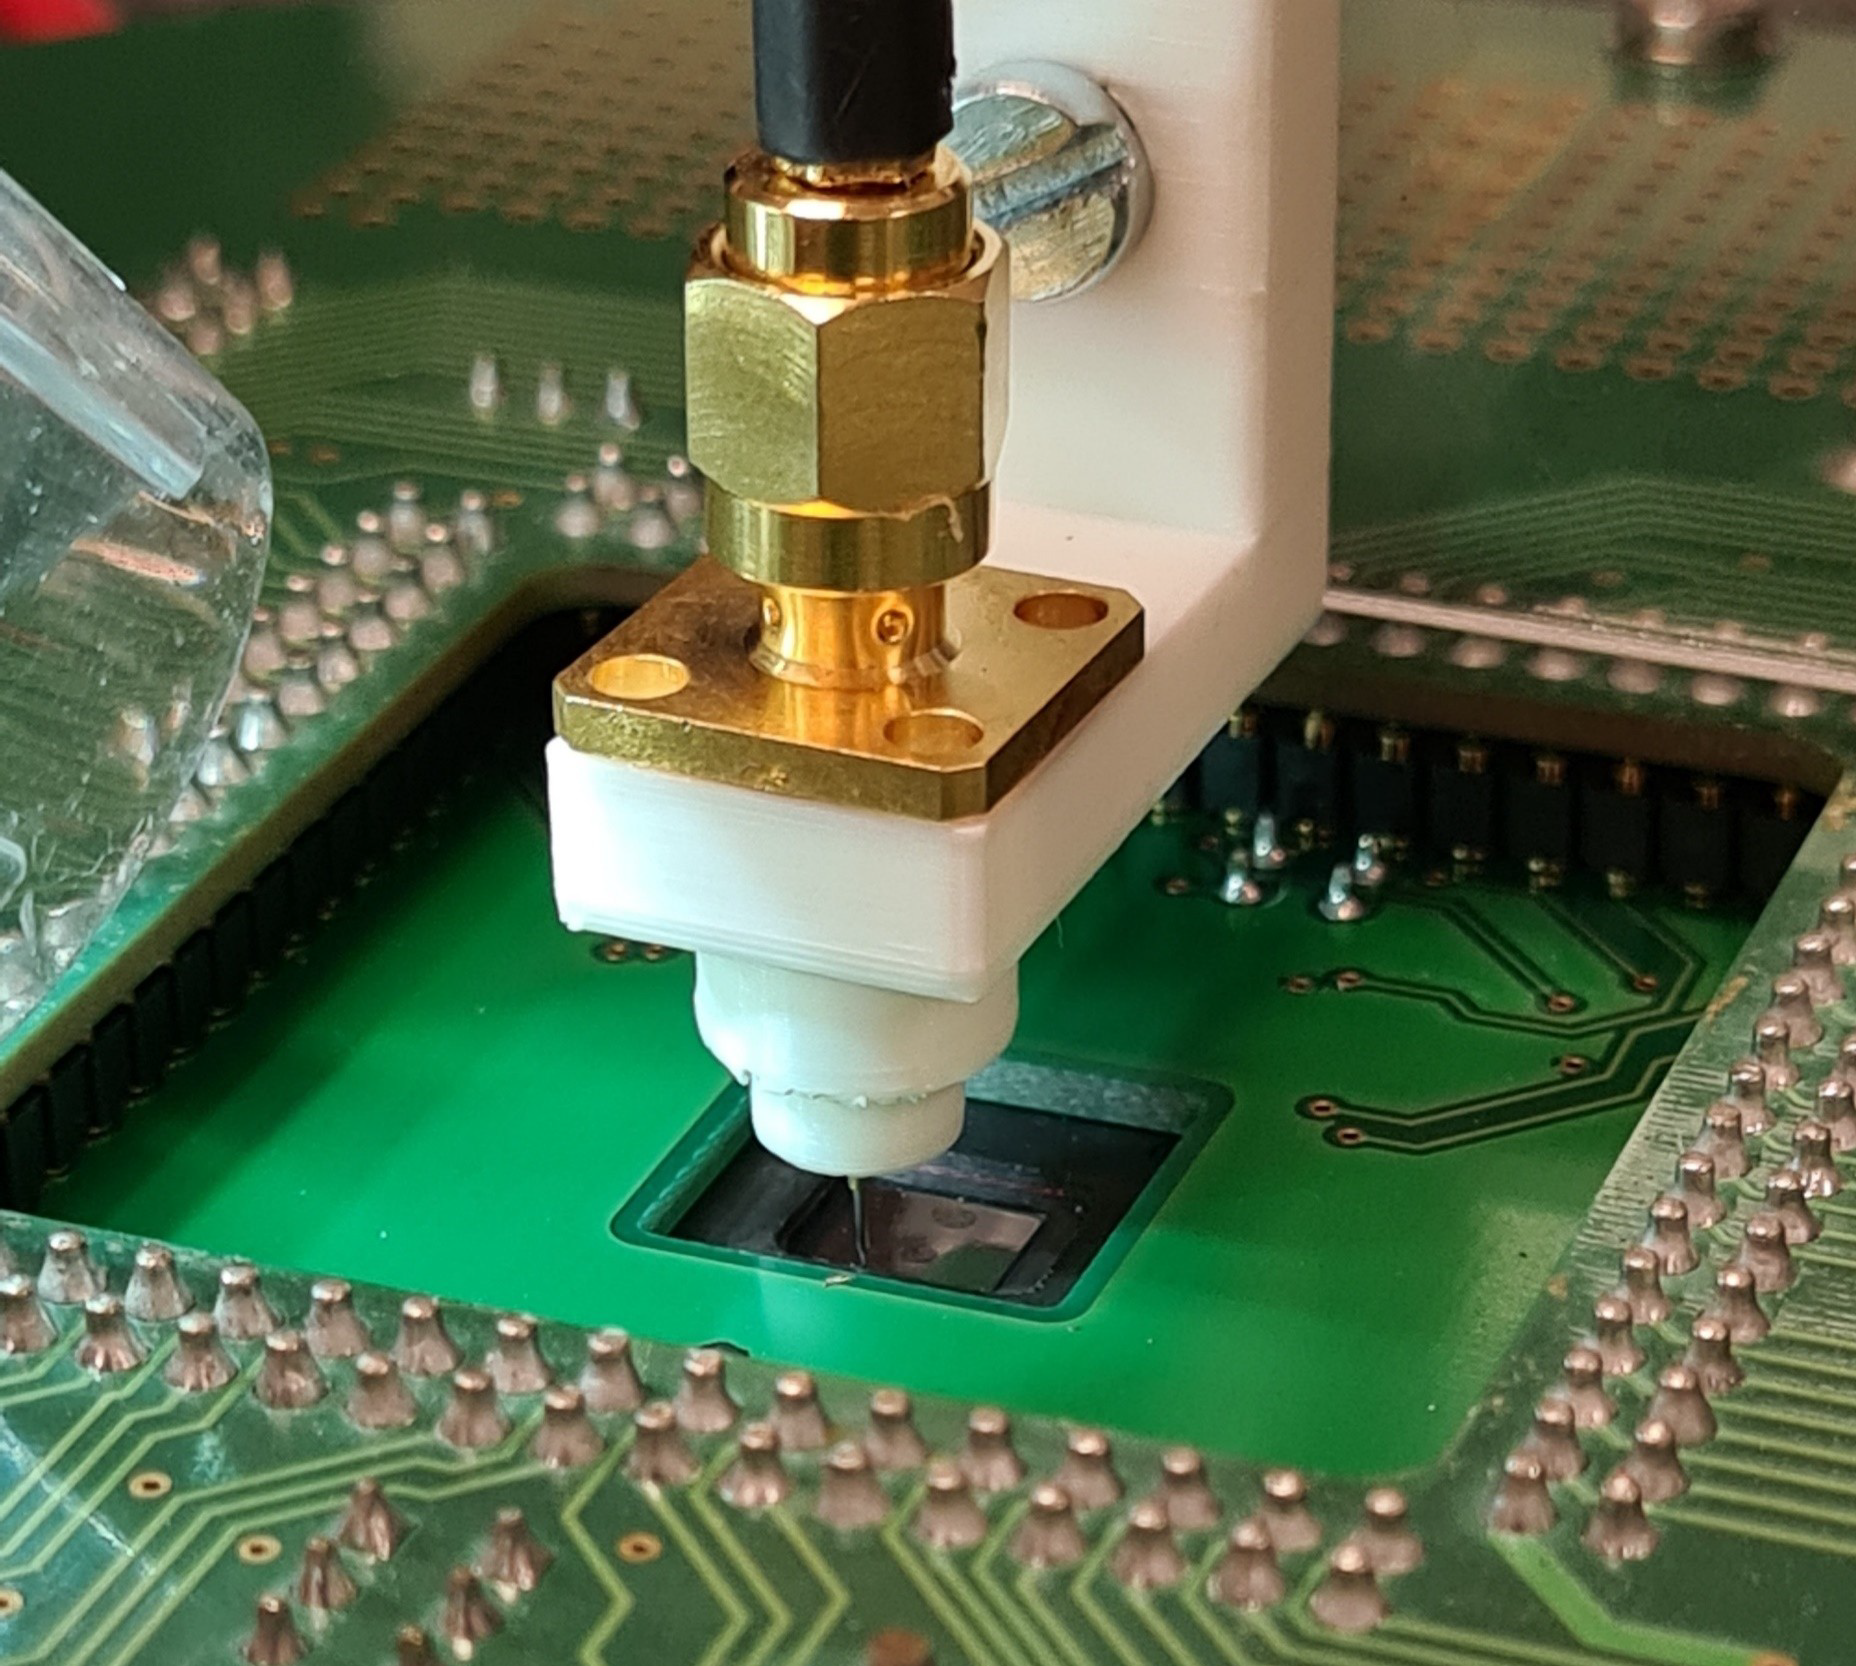
\includegraphics[width=\textwidth]{sondeBBI_loin_raw.png}
            \end{figure}
            \begin{figure}
                \includegraphics[width=\textwidth]{pointeBBI2.png}
            \end{figure}
        \end{column}

        \barsep

        \begin{column}{0.5\textwidth}
            \centering
%            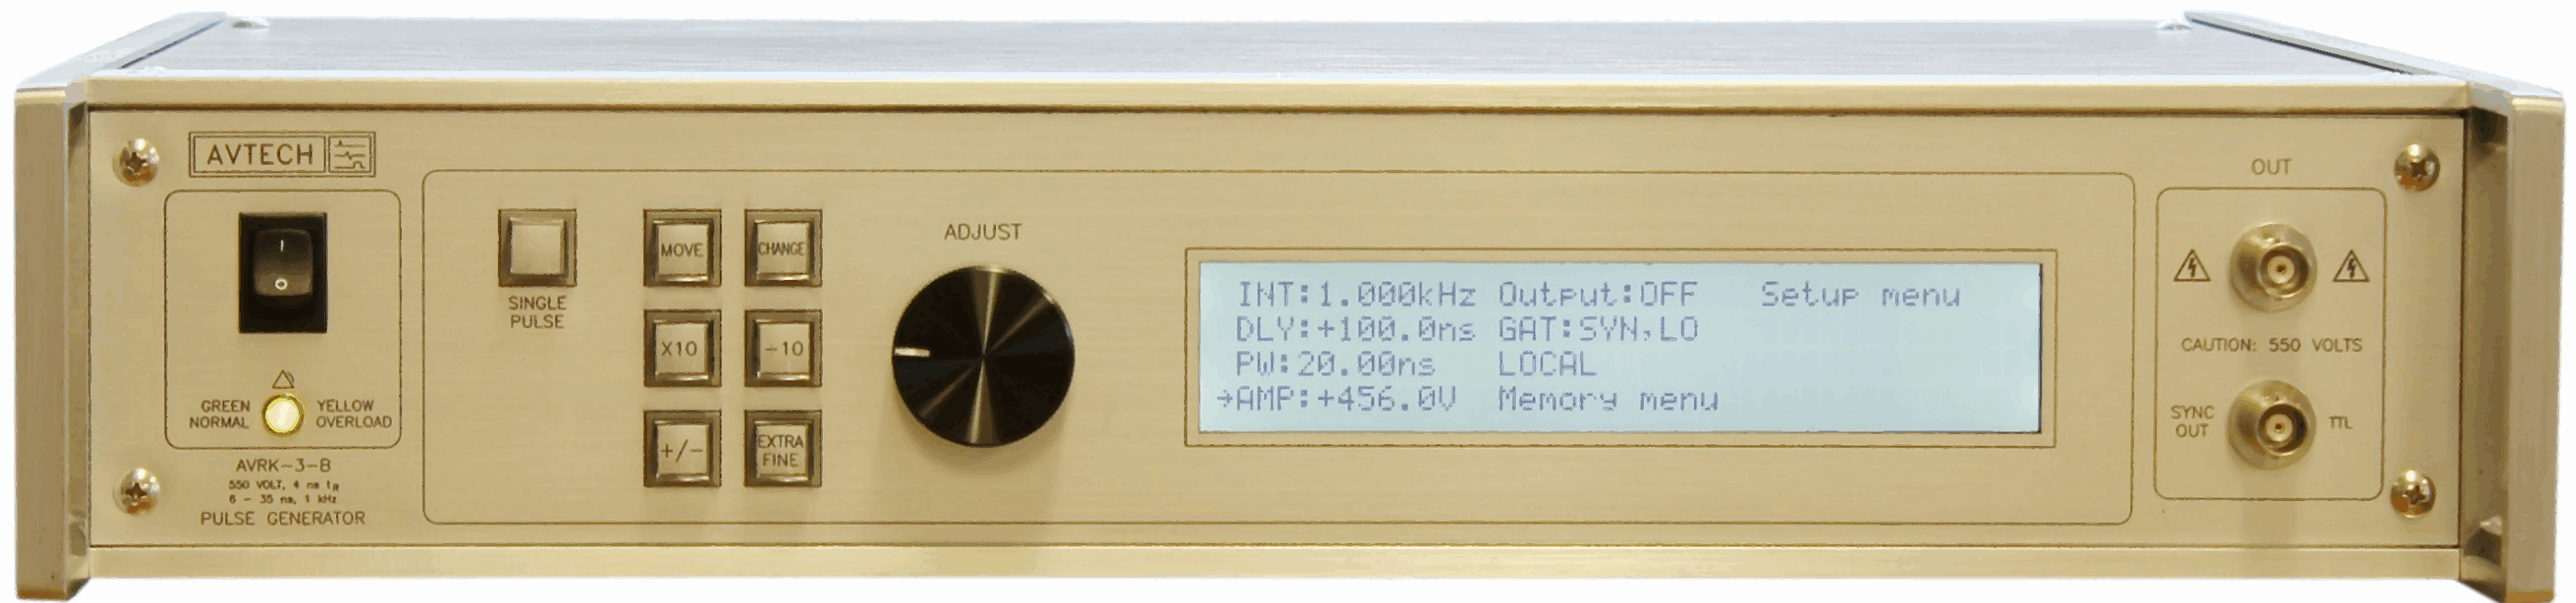
\includegraphics[width=0.9\textwidth]{avrk4b.pdf}
        \end{column}

    \end{columns}
\end{frame}
%    
\section{BETTER PRACTICES FOR BODY BIASING INJECTION}
\begin{frame}
    \frametitle{State-of-the-art BBI platform: limiting factors}
    \begin{columns}
        \begin{column}{0.67\textwidth}
            \begin{textblock*}{120mm}(5mm, 20mm)
                • Impedance mismatch → Ringing and set-point error\\
                • Floating grounds → Set-point error
            \end{textblock*}
            \begin{textblock*}{65mm}(20mm, 31mm)
                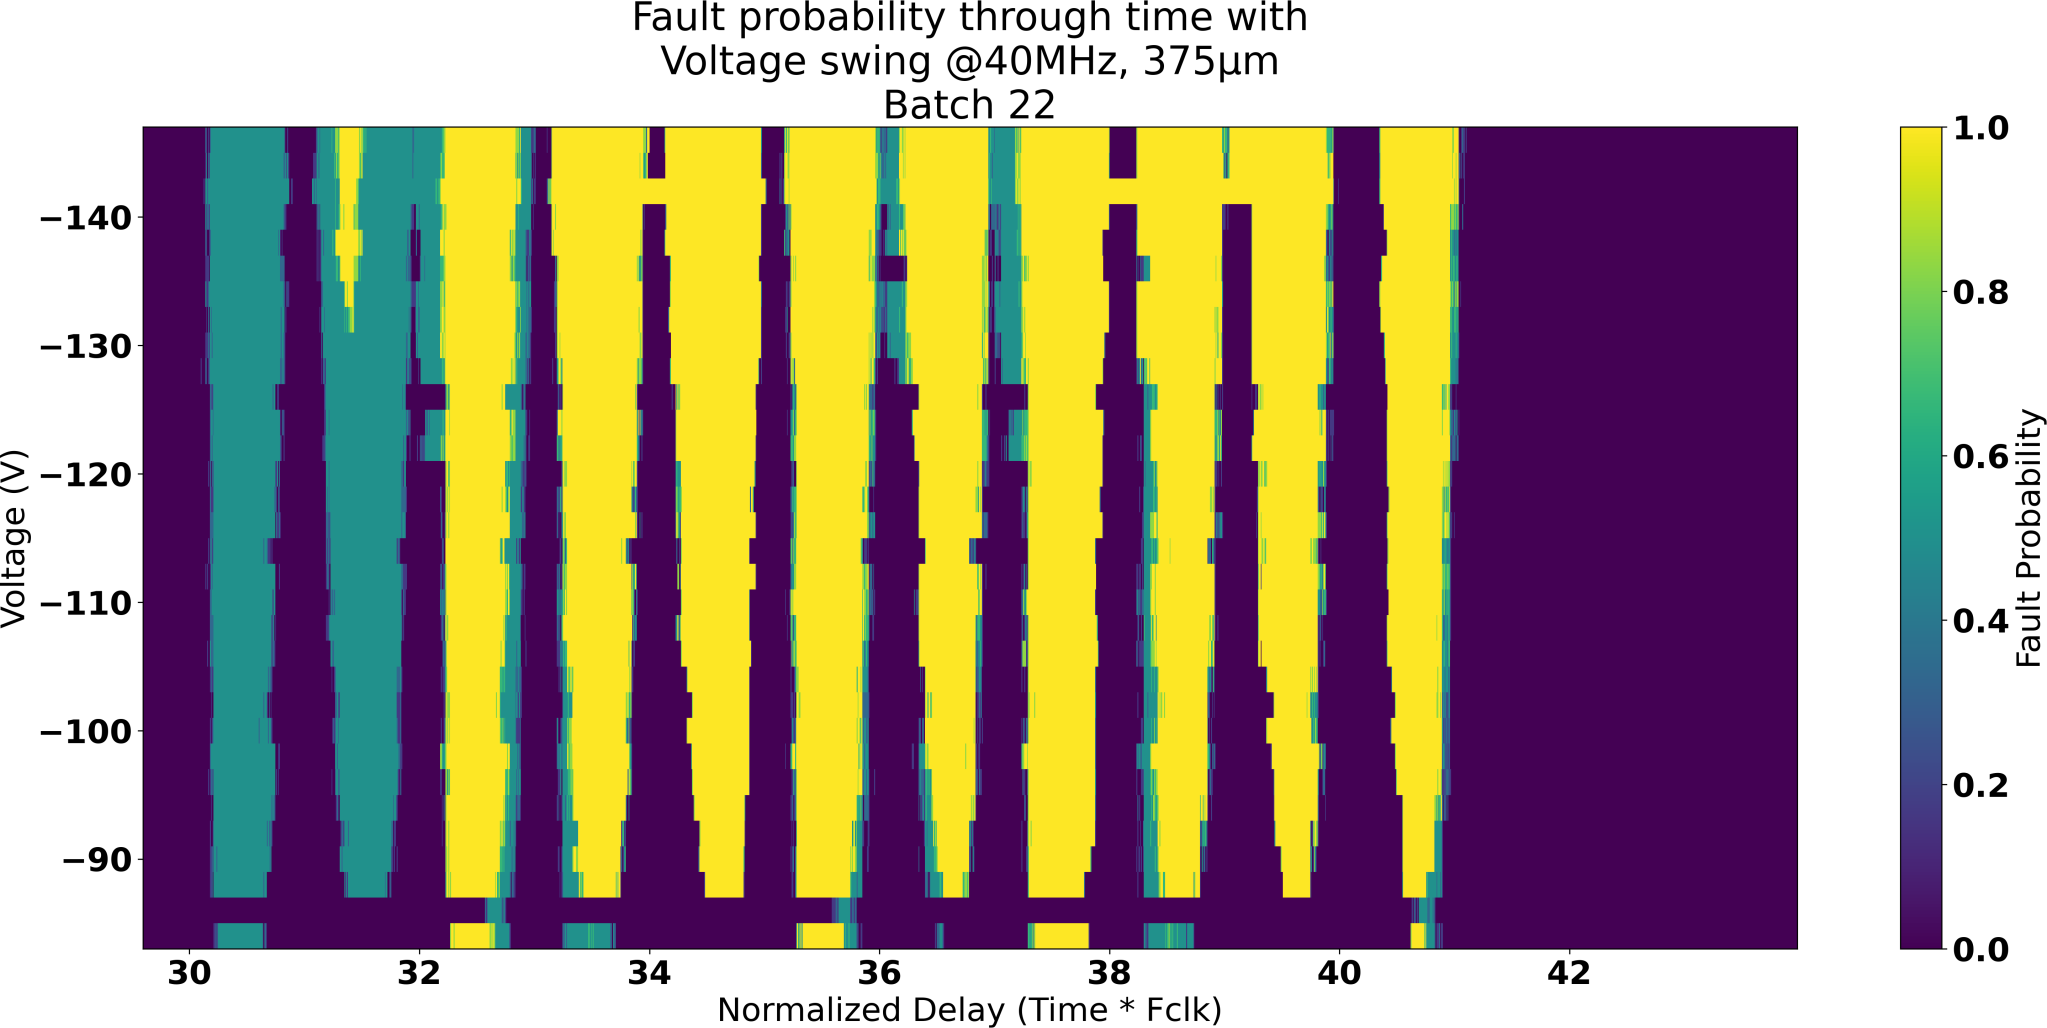
\includegraphics[width=\textwidth]{probafautes0.png}
            \end{textblock*}
            \begin{textblock*}{65mm}(20mm, 65mm)
                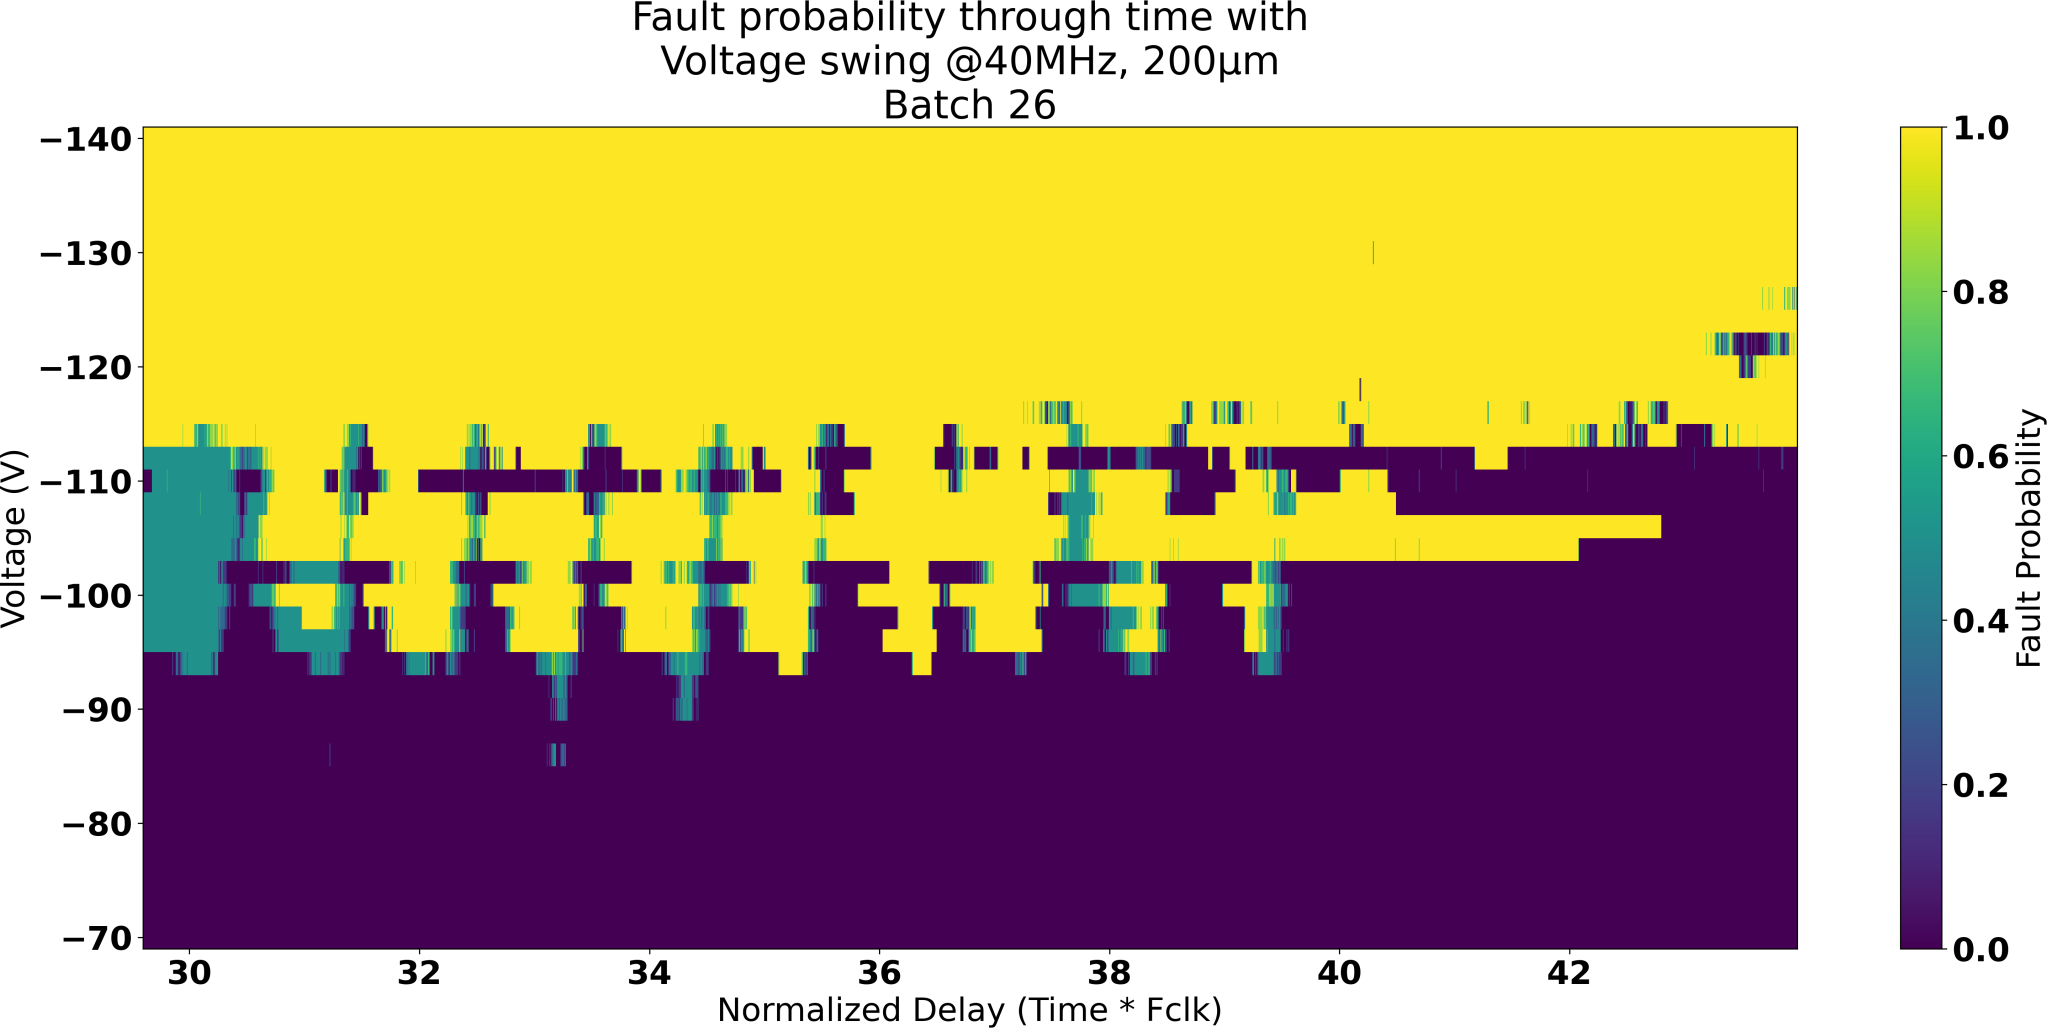
\includegraphics[width=\textwidth]{probafautes1.png}
            \end{textblock*}
        \end{column}
        %   Barre centrale
        \begin{textblock*}{1mm}(100mm, 20mm)
            
\begin{tikzpicture}
                \draw[-, black, line width=0.5mm] (0, 0) -- (0, 7.5);
            \end{tikzpicture}
        \end{textblock*}
        \begin{column}{0.33\textwidth}
            \centering
            \begin{figure}
                
\includegraphics[width=1.0\textwidth]{model0Probe.pdf}
            \end{figure}
            \vspace{-0.5cm}
            \begin{figure}
                \includegraphics[width=0.9\textwidth]{S1P.pdf}\\
                \includegraphics[width=0.9\textwidth]{S1G.pdf}
            \end{figure}
        \end{column}
    \end{columns}
\end{frame}

%    
\begin{frame}
    \frametitle{Enhanced BBI platform}
%    Schéma
    \begin{textblock*}{60mm}(48mm, 16mm)
        \includegraphics[width=\textwidth]{model2ProbeManuscrit.pdf}
    \end{textblock*}
%   Flèche gauche
    \begin{textblock*}{1mm}(28mm, 24mm)
        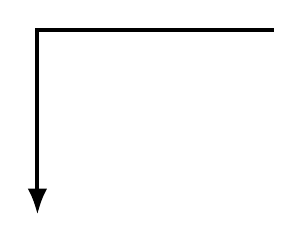
\begin{tikzpicture}
                \draw[-Latex, black, line width=0.5mm] (0, 0) -| (-3, -2.35);
            \end{tikzpicture}
    \end{textblock*}
%   Flèche droite
    \begin{textblock*}{1mm}(99mm, 35.0mm)
        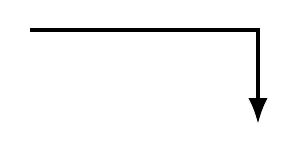
\begin{tikzpicture}
            \draw[-Latex, black, line width=0.5mm] (0, 0) -| (2.9, -1.2);
        \end{tikzpicture}
    \end{textblock*}
%    Courant
    \begin{textblock*}{60mm}(98mm, 49mm)
        \includegraphics[width=\textwidth]{S2G.pdf}
    \end{textblock*}
%    Pulse
    \begin{textblock*}{60mm}(2mm, 49mm)
        \includegraphics[width=\textwidth]{S2P.pdf}
    \end{textblock*}
%    impMatchGen
    \begin{textblock*}{28mm}(67mm, 51mm)
        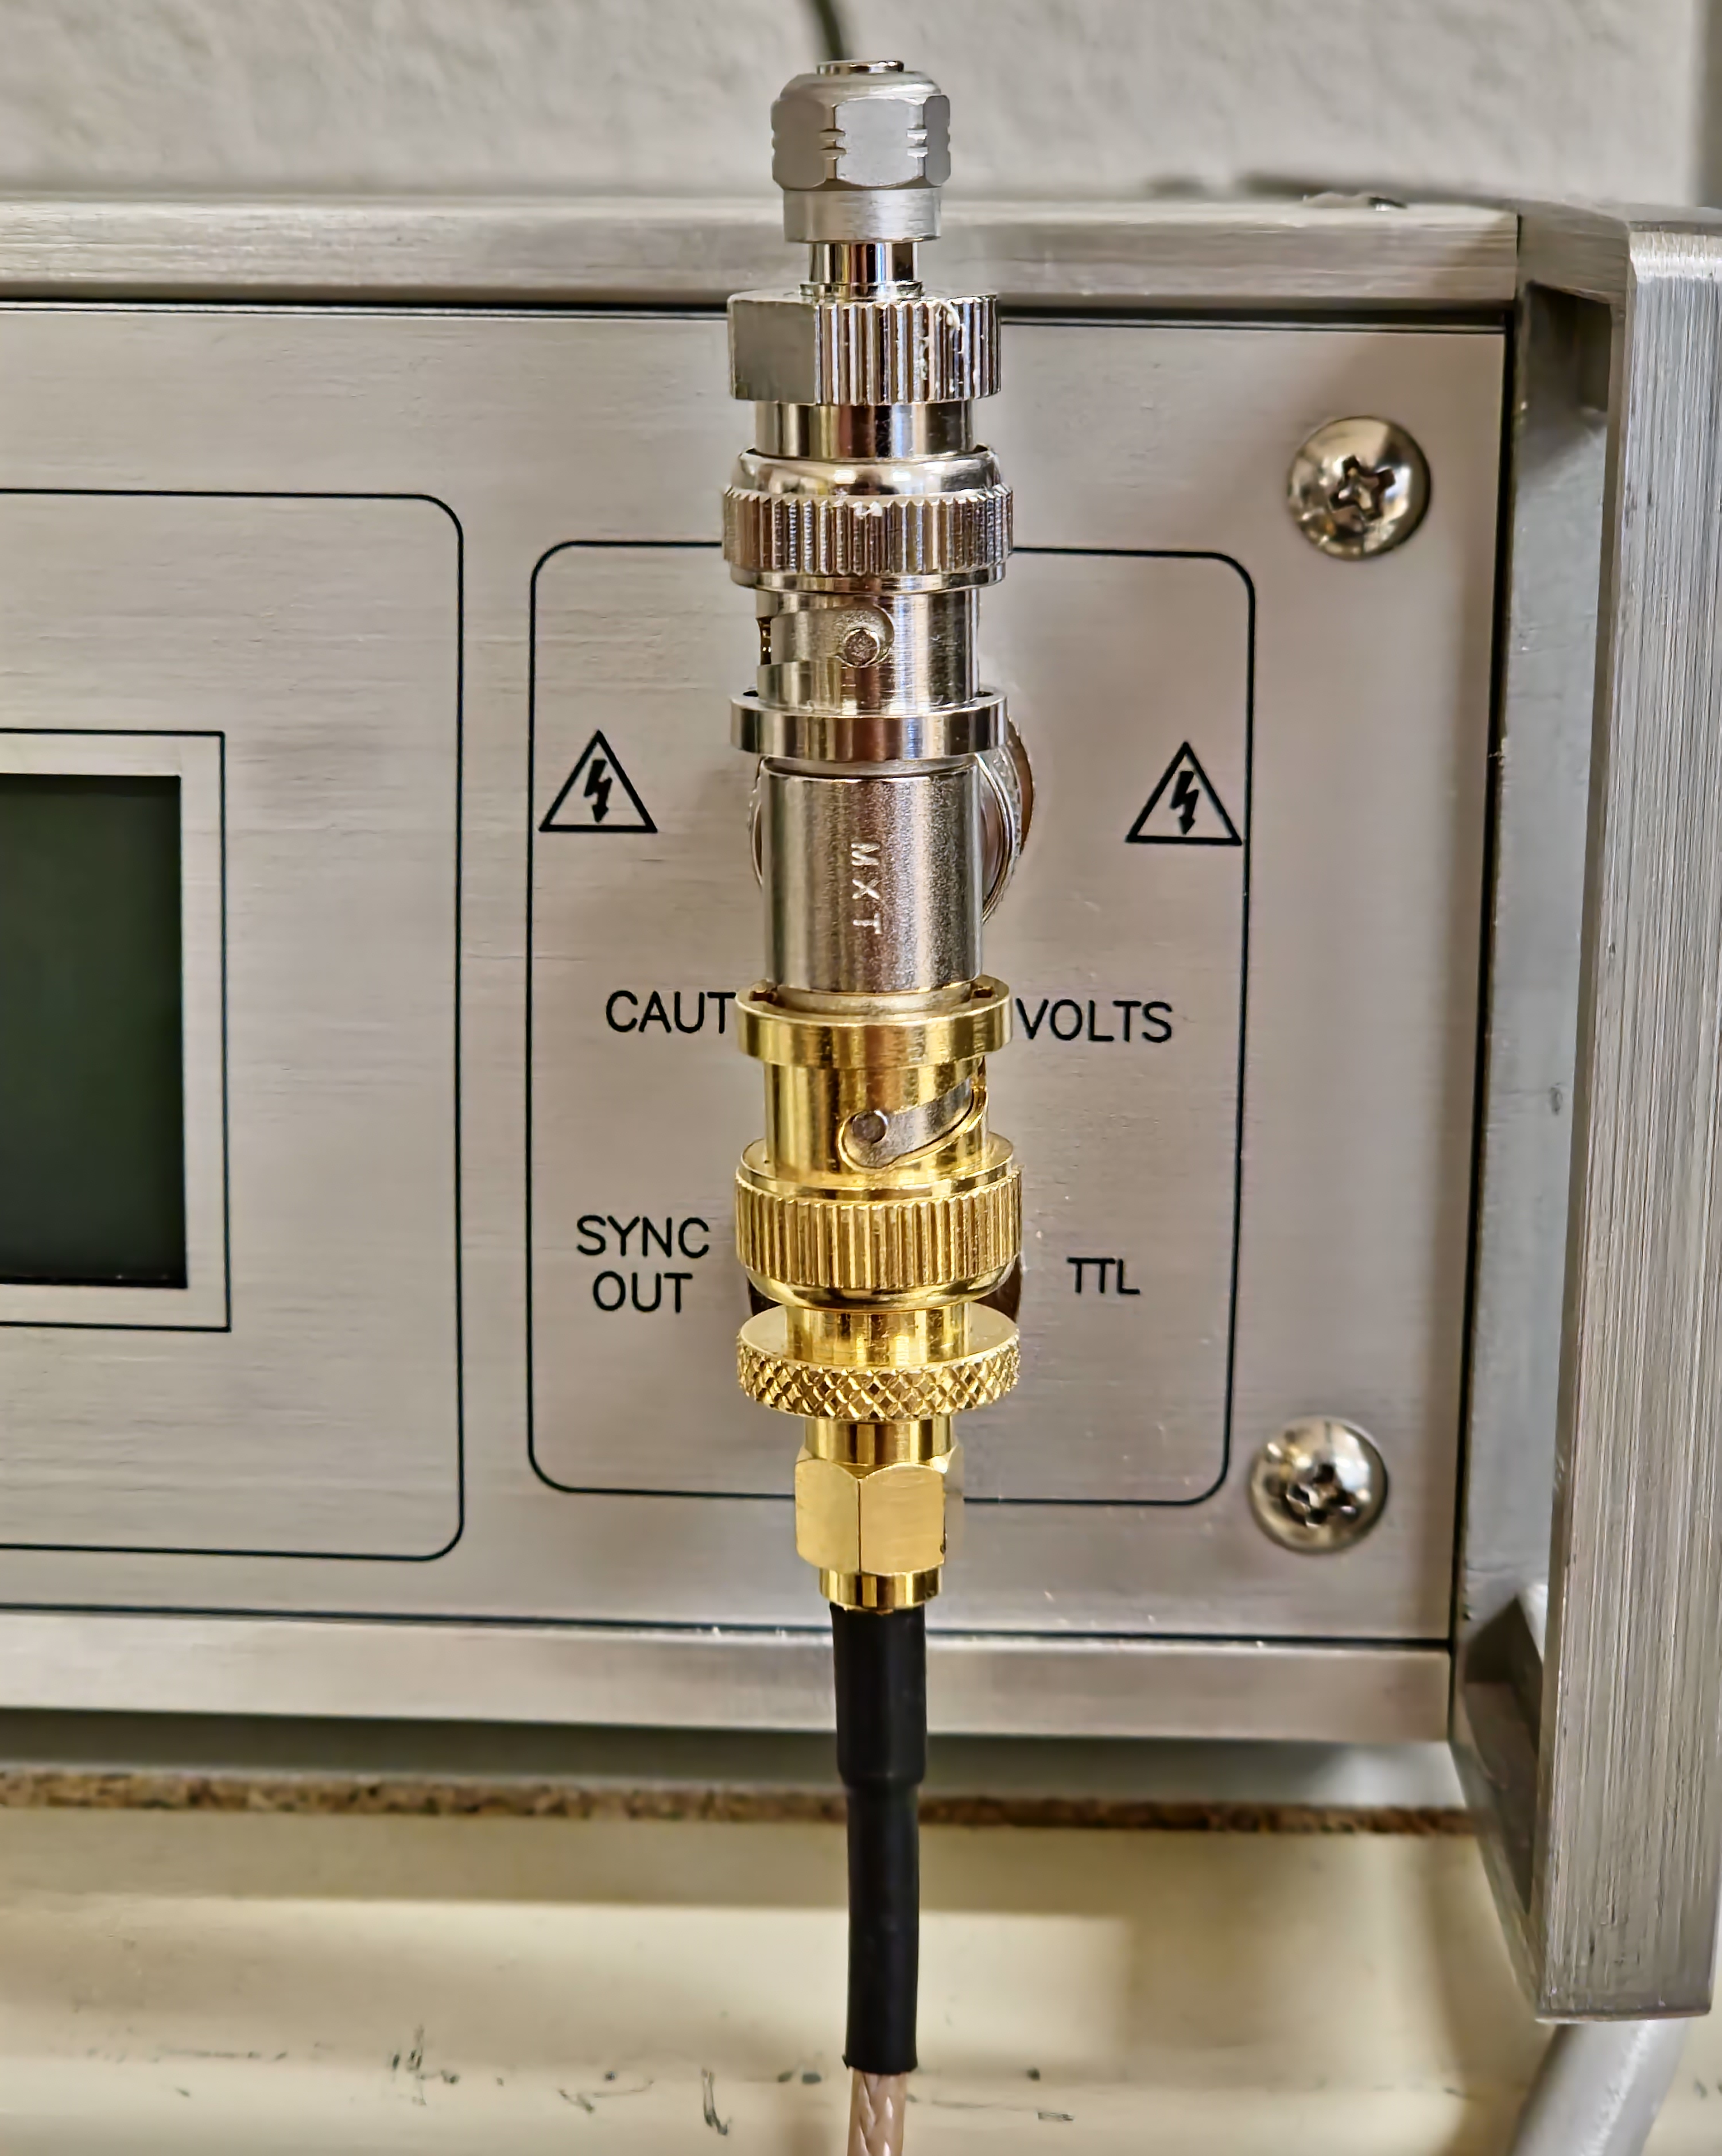
\includegraphics[width=\textwidth]{impMatchPicture.jpg}
    \end{textblock*}
%    cercle image
    \begin{textblock*}{1mm}(75.3mm, 50mm)
        
\begin{tikzpicture}
            \draw[line width=0.5mm, color=red] circle (0.3);
        \end{tikzpicture}
    \end{textblock*}
%   Flèche image
    \begin{textblock*}{1mm}(66mm, 34mm)
        
\begin{tikzpicture}
            \draw[-Latex, red, line width=0.5mm] (0, 0) |- (0.8, -1.9);
        \end{tikzpicture}
    \end{textblock*}
\end{frame}

%    
\begin{frame}
    \frametitle{BBI in practice}
    \framesubtitle{Actual results: voltage pulse and IC ground current}
%    \centering
    \begin{columns}
        \begin{column}{0.6\textwidth}
            \centering
%            \includegraphics[width=\textwidth]{realPulsesComparisons.pdf}
        \end{column}

%        \barsep

        \begin{column}{0.4\textwidth}
            \centering
            Default platform:
            \begin{itemize}
                \item -108 \% pulse undershoot;
                \item 275 \% pulse width overshoot;
                \item Obvious ringing.
            \end{itemize}
            Enhanced platform:
            \begin{itemize}
                \item -31 \% undershoot;
                \item Matched pulse width;
                \item Less ringing.
            \end{itemize}
        \end{column}
    \end{columns}

\end{frame}

%    
\begin{frame}
    \frametitle{Enhanced BBI platform benefits}
    \framesubtitle{Giraud's single bit fault attack}
%    \barhoriz{10mm}
%    \vspace{0.05cm}
%    
\includegraphics[width=0.32\textwidth]{model0Probe.pdf}
%    \includegraphics[width=0.32\textwidth]{aesFastGndOnly.pdf}
%    \vspace{-0.4cm}
%    \par
%    \rule{\framewidth}{0.5mm}
%    \par
%    \vspace{0.1cm}
%    \includegraphics[width=0.32\textwidth]{model2ProbeManuscrit.pdf}
%    \includegraphics[width=0.32\textwidth]{aesFastImpGnd.pdf}
    \begin{columns}
        \begin{column}{0.32\textwidth}
            
\includegraphics[width=\textwidth]{model0Probe.pdf}
            \vspace{0.09cm}
            \par
            \vspace{0.09cm}
            \includegraphics[width=\textwidth]{model2ProbeManuscrit.pdf}
        \end{column}

        \begin{column}{0.32\textwidth}
            \includegraphics[width=\textwidth]{aesFastGndOnly.pdf}
            \vspace{0.02cm}
            \par
            \vspace{0.02cm}
            \includegraphics[width=\textwidth]{aesFastImpGnd.pdf}
        \end{column}

        \begin{column}{0.32\textwidth}
            Unsuccessful Giraud's DFA
            \vspace{1.3cm}
            \par
            \vspace{1.3cm}
            Successful Giraud's DFA
        \end{column}
    \end{columns}
\end{frame}

%    
\begin{frame}
    \frametitle{Giraud's single bit fault attack}
    \framesubtitle{Results}
    \includegraphics[width=\textwidth]{giraud__7N.pdf}
    \vspace{0.6cm}
    \begin{itemize}
        \setlength\itemsep{1em}
        \item 14 bytes out of 16 found thanks to the Giraud's DFA;
        \item 2 remaining bytes found thanks to brute force.
    \end{itemize}

\end{frame}

%    
\begin{frame}
    \frametitle{TITLE}
    \framesubtitle{SUBTITLE}

\end{frame}


%    IGNORE FOLLOWING
%    
\begin{frame}
    \frametitle{Bulk substrate types}
%    \framesubtitle{SUBTITLE}
%    \hfill
    \includegraphics[width=0.4\textwidth]{DUAL.pdf}
    \hfill
    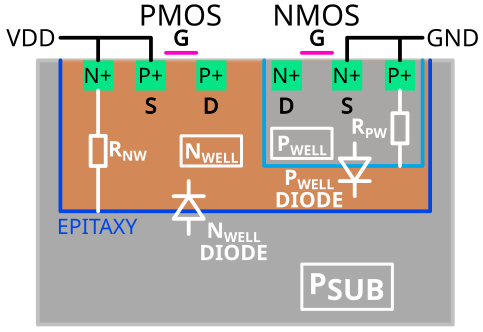
\includegraphics[width=0.4\textwidth]{TRIPLE.pdf}
    \hfill

\end{frame}

%    
\begin{frame}
    \frametitle{Standard-cell original models}
    %    \framesubtitle{SUBTITLE}
    %    \hfill
    \includegraphics[width=0.4\textwidth]{dualWellEmfi.png}
    \hfill
    \includegraphics[width=0.4\textwidth]{tripleWellEmfi.png}
    \hfill

\end{frame}

%    
\begin{frame}
    \frametitle{Standard-cell model substrate improvement}
%    \framesubtitle{SUBTITLE}
%    \includegraphics[width=0.5\textwidth]{substrateSubdivision_88.png}
%    \includegraphics[width=0.5\textwidth]{dualWell_no_7c_Eevee.png}
%    \includegraphics[width=0.5\textwidth]{tripleWell_no_7c_Eevee.png}
    \begin{columns}
        \begin{column}{0.35\textwidth}
            \includegraphics[width=\textwidth]{substrateSubdivision_88.png}
        \end{column}
        \begin{column}{0.3\textwidth}
            \includegraphics[width=\textwidth]{dualWell_no_7c_Eevee.png}
        \end{column}
        \begin{column}{0.3\textwidth}
            \includegraphics[width=\textwidth]{tripleWell_no_7c_Eevee.png}
        \end{column}
    \end{columns}

\end{frame}

%    
\begin{frame}
    \frametitle{IC generation}
%    \framesubtitle{SUBTITLE}
    \begin{columns}
        \begin{column}{0.5\textwidth}
            \includegraphics[width=\textwidth]{resultingSimulated_ic.png}
        \end{column}
        \begin{column}{0.5\textwidth}
            \begin{itemize}
                \item Item
                \item Item
                \item Item
                \item Item
                \item Item
            \end{itemize}
        \end{column}
    \end{columns}

\end{frame}

%    
\begin{frame}
    \frametitle{Generator model}
%    \framesubtitle{SUBTITLE}

\end{frame}

%    IGNORE PREVIOUS

    
\section{SIMULATION RESULTS}
\begin{frame}{Simulation results}
    What we observe:
    \begin{itemize}
        \item Dual-well;
        \item Triple-well;
        \item Picture at the apex of the pulse;
        \item $550 \; \mu m \; (W) \; \times \; 450 \; \mu m \; (D) \; \times \; 140 \; \mu m \; (T)$: integrated circuit → 1620 SCS;
    \end{itemize}
    Simulation conditions:
    \begin{itemize}
        \item Voltage pulse amplitude: -300 V;
        \item Voltage pulse width: 20 ns;
        \item Rise and fall times: 8 ns;
        \item Approximate impedance matching.
    \end{itemize}
\end{frame}

\begin{frame}
%    [trim={left bottom right top},clip]
    \frametitle{Simulation results: Dual-Well}
    %    \framesubtitle{SUBTITLE}
    \begin{columns}
        \begin{column}{0.3\textwidth}
            \vspace{-1mm}
            \begin{figure}
                \includegraphics[width=\textwidth]{vddMgndManuscrit.pdf}
                \caption{\centering PS voltage distribution}
            \end{figure}
            \vspace{-2mm}
            \begin{figure}
                \includegraphics[width=\textwidth]{iEpiDualWellManuscrit.pdf}
                \caption{\centering Epitaxy current distribution}
            \end{figure}
        \end{column}

        \begin{column}{0.6\textwidth}
            \vspace{-2mm}
            \begin{figure}
                \includegraphics[width=\textwidth]{iSubcManuscrit.pdf}
                \caption{Substrate current distribution}
            \end{figure}
            \vspace{-1mm}
            \begin{figure}
                \includegraphics[trim={0mm 0mm 0mm 13mm}, clip, width=\textwidth]{CurrentDistributionNormT140eT10_ExcDw.pdf}
                \caption{Per-layer normalized substrate current density}
            \end{figure}
        \end{column}
    \end{columns}
\end{frame}

    
\begin{frame}
    %    [trim={left bottom right top},clip]
    \frametitle{Simulation results: Triple-Well}
    \begin{columns}
        \begin{column}{0.3\textwidth}
            \vspace{-1mm}
            \begin{figure}
                \includegraphics[width=\textwidth]{vddMgndManuscritTw.pdf}
                \caption{\centering PDN (VDD - GND)}
            \end{figure}
            \vspace{-2mm}
            \begin{figure}
                \includegraphics[width=\textwidth]{iEpiTripleWellManuscrit.pdf}
                \caption{\centering Epitaxy current distribution}
            \end{figure}
        \end{column}

        \begin{column}{0.6\textwidth}
            \vspace{-2mm}
            \begin{figure}
                \includegraphics[width=\textwidth]{iSubcManuscritTws.pdf}
                \caption{Substrate current distribution}
            \end{figure}
            \vspace{2mm}
            \begin{figure}
                \includegraphics[trim={0mm 0mm 0mm 13mm}, clip, width=\textwidth]{CurrentDistributionNormT140eT10_ExcTw.pdf}
                \caption{Per-layer normalized substrate current density: }
            \end{figure}
%            \centering 186 µm diameter mid-height
        \end{column}
    \end{columns}
\end{frame}

\begin{frame}{Dual-well vs Triple-well}
    \Large Differences between Dual-well and Triple-well circuits:
    \begin{table}[]
        \resizebox{\framewidth}{!}{
        \begin{tabular}{
                >{\columncolor[HTML]{EFEFEF}}c
                >{\columncolor[HTML]{EFEFEF}}c cc
                >{\columncolor[HTML]{FFFC9E}}c c}
            \cellcolor[HTML]{DAE8FC}                            & \cellcolor[HTML]{DAE8FC}                           & \multicolumn{3}{c}{\cellcolor[HTML]{DAE8FC}Coupling}                                                                                    & \cellcolor[HTML]{DAE8FC}                           \\
            \multirow{-2}{*}{\cellcolor[HTML]{DAE8FC}Substrate} & \multirow{-2}{*}{\cellcolor[HTML]{DAE8FC}Polarity} & \cellcolor[HTML]{DAE8FC}NMOS                      & \cellcolor[HTML]{DAE8FC}PMOS                      & \cellcolor[HTML]{DAE8FC}Circuit & \multirow{-2}{*}{\cellcolor[HTML]{DAE8FC}Danger}   \\
            Dual-well                                           & Negative                                           & \cellcolor[HTML]{FFFC9E}{\color[HTML]{000000} DC} & \cellcolor[HTML]{9AFF99}AC                        & {\color[HTML]{000000} DC}       & \cellcolor[HTML]{FFCCC9}{\color[HTML]{000000} \skull\skull\skull} \\
            Dual-well                                           & Positive                                           & \cellcolor[HTML]{FFFC9E}{\color[HTML]{000000} DC} & \cellcolor[HTML]{FFFC9E}{\color[HTML]{000000} DC} & {\color[HTML]{000000} DC}       & \cellcolor[HTML]{FD6864}\skull\skull\skull\skull        \\
            Triple-well                                         & Negative                                           & \cellcolor[HTML]{9AFF99}AC                        & \cellcolor[HTML]{9AFF99}AC                        & \cellcolor[HTML]{9AFF99}AC      & \cellcolor[HTML]{96FFFB}\skull                          \\
            Triple-well                                         & Positive                                           & \cellcolor[HTML]{9AFF99}AC                        & \cellcolor[HTML]{FFFC9E}{\color[HTML]{000000} DC} & {\color[HTML]{000000} DC}       & \cellcolor[HTML]{FFCCC9}{\color[HTML]{000000} \skull\skull\skull}
        \end{tabular}}
    \end{table}
\end{frame}

    
\begin{frame}
    \frametitle{Simulation results verification}
%    \framesubtitle{SUBTITLE}
    \begin{columns}
        \begin{column}{0.5\textwidth}
            \begin{figure}
                \centering
                \includegraphics[width=\textwidth]{pos_neg_IGND.pdf}
                \caption{$V_{PULSE}=-70\;V; \; PW = 20\; ns$}
            \end{figure}
        \end{column}

        \begin{column}{0.425\textwidth}
            \begin{figure}
                \centering
                \includegraphics[width=\textwidth]{stmPhotoImshow.pdf}
            \end{figure}
        \end{column}
    \end{columns}

\end{frame}

    
\section{SIMULATION FLOW FOLLOW-UP: HOW FAULTS OCCUR?}

%\begin{frame}{SCS incomplete models: how faults occur?}
%    \begin{center}
%        \onslide<1-2>{\huge To understand how faults occur}
%        \onslide<2-2>{\\↓\\
%        We need to consider the logic inside the IC}
%    \end{center}
%\end{frame}

\begin{frame}{SCS incomplete models: how to consider logic function?}
    \begin{textblock*}{5cm}(5mm, 20mm)
        \includegraphics[width=1.0\textwidth]{tripleWell_no_7c_Eevee.png}
    \end{textblock*}
%    \tikz \draw [arrows = {-Stealth[length=10pt, inset=5pt]}] (0,0) -- (1,0);
    \begin{textblock*}{1cm}(60mm, 28mm)
        \tikz [line width=1mm]\draw [arrows = {-Stealth[length=10pt]}] (0,0) -- (2.65,0);
    \end{textblock*}

    \begin{textblock*}{5cm}(91.9mm, 25.38mm)
        \includegraphics[width=1.0\textwidth]{logicGates.pdf}
    \end{textblock*}

    \begin{textblock*}{1cm}(115.77mm, 33.65mm)
        \tikz [line width=1mm]\draw [arrows = {-Stealth[length=10pt]}] (0,0) -- (0,-1);
    \end{textblock*}

    \begin{textblock*}{1cm}(96mm, 45mm)
%        \tikz [line width=1mm]\draw [decorate, decoration={brace}] (0, 0) -- (3, 0)
        
\begin{tikzpicture}
            \draw[decorate, decoration={brace, amplitude=10pt}, black, line width=2pt] (0, 0) -- (4.15, 0.0);
        \end{tikzpicture}
    \end{textblock*}

    \begin{textblock*}{5cm}(90mm, 50mm)
        \includegraphics[width=1.0\textwidth]{ivx3New.pdf}
    \end{textblock*}
\end{frame}

%    
\begin{frame}{How faults occur under BBI?}{Dual-well inverters}
    \begin{columns}
        \begin{column}{0.32\textwidth}
            \begin{figure}
                \includegraphics[width=1.0\textwidth]{ivx3NewNoSignals.pdf}
            \end{figure}
        \end{column}
        \begin{column}{0.36\textwidth}
            \begin{figure}
                \includegraphics[width=1.0\textwidth]{logic_gates_solo_M0_DW.pdf}
            \end{figure}
        \end{column}
        \begin{column}{0.32\textwidth}
            \begin{figure}
                \includegraphics[width=1.0\textwidth]{logic_gates_solo_M0_DW_n2.pdf}
            \end{figure}
        \end{column}
    \end{columns}
\end{frame}

\begin{frame}{How faults occur under BBI?}{Triple-well inverters}
    \begin{columns}
        \begin{column}{0.32\textwidth}
            \begin{figure}
                \includegraphics[width=1.0\textwidth]{ivx3New.pdf}
            \end{figure}
        \end{column}
        \begin{column}{0.34\textwidth}
            \begin{figure}
                \includegraphics[width=1.0\textwidth]{logic_gates_solo_M0_TW.pdf}
            \end{figure}
        \end{column}
        \begin{column}{0.34\textwidth}
            \begin{figure}
                \includegraphics[width=1.0\textwidth]{logic_gates_solo_M0_TW_n2.pdf}
            \end{figure}
        \end{column}
    \end{columns}
\end{frame}

%    
\begin{frame}{How faults occur under BBI?}{Fault model}
    \Large Data dependent faults:
    \begin{itemize}
        \item Circuits leaks more info;
        \item Can lead to safe-error attack.
    \end{itemize}
\end{frame}

%    
\section{SUBSTRATE THINNING ANALYSIS}
\begin{frame}{Substrate thinning in a BBI context}
    \begin{center}
        \Large
        In Laser Fault Injection, substrate thinning has been proven useful\\
        Is it the case concerning BBI?
    \end{center}
    \vspace{5mm}
    \large
    Section agenda:
    \begin{itemize}
        \item Geometric approach
        \item Electrical simulation approach
        \item Experimental validation
    \end{itemize}
\end{frame}

%    
\begin{frame}
    \frametitle{Geometric approach}
    \begin{columns}
        \begin{column}{0.5\textwidth}
            \begin{figure}
                \includegraphics[width=\textwidth]{geomCrossViewNew.pdf}
            \end{figure}
        \end{column}
        \begin{column}{0.5\textwidth}
            \begin{figure}
                \includegraphics[width=\textwidth]{geomCrossViewThinNew.pdf}
            \end{figure}
        \end{column}
    \end{columns}
\end{frame}

\begin{frame}
    \frametitle{Geometric approach}
    \begin{columns}
        \begin{column}{0.5\textwidth}
            \begin{figure}
                \includegraphics[width=\textwidth]{geomCrossViewNew.pdf}
            \end{figure}
        \end{column}
        \begin{column}{0.5\textwidth}
            \begin{figure}
                \includegraphics[width=\textwidth]{geomCrossViewThinNew2.pdf}
            \end{figure}
        \end{column}
    \end{columns}
\end{frame}

\begin{frame}{Geometric approach outcomes}
    \begin{enumerate}
        \setlength\itemsep{2em}
        \item Thinning the substrate → Reduce the voltage pulse for a given susceptibility area;
        \item Thinning the substrate → Susceptibility area increases at constant voltage;
        \item Thinning the substrate → No improvement in resolution.
    \end{enumerate}
\end{frame}

%    
\begin{frame}{Simulation approach}
    What we observe:
    \begin{itemize}
        \item Dual-well substrate IC;
        \item Picture at the apex of the pulse;
        \item $550 \; \mu m \; (W) \; \times \; 450 \; \mu m \; (D)$: integrated circuit → 1620 SCS;
        \item $140 \; \mu m \; (T)$ IC;
        \item $60 \; \mu m \; (T)$ IC;
    \end{itemize}
    Simulation conditions:
    \begin{itemize}
        \item Voltage pulse amplitude: -300 V;
        \item Voltage pulse width: 20 ns;
        \item Rise and fall times: 8 ns.
    \end{itemize}
\end{frame}

\begin{frame}
    \frametitle{Simulation approach}
    %    \framesubtitle{SUBTITLE}
    \begin{columns}
        \begin{column}{0.5\textwidth}
            \begin{figure}
                \includegraphics[width=\textwidth]{thinning140um.pdf}
                \par
                \includegraphics[width=\textwidth]{VoltageDistributionNormT140eT10_ExcDw.pdf}
            \end{figure}
        \end{column}

        \begin{column}{0.5\textwidth}
            \begin{figure}
                \includegraphics[width=\textwidth]{thinning60um.pdf}
                \par
                \includegraphics[width=\textwidth]{VoltageDistributionNormT60eT10_ExcDw.pdf}
            \end{figure}
        \end{column}
    \end{columns}

\end{frame}
%VoltageDistributionNormT60eT10_ExcDw.pdf
%VoltageDistributionNormT140eT10_ExcDw.pdf
%thinning140um
%thinning60um

%    
\begin{frame}
    \frametitle{A few words on substrate thinning techniques}
    AJOUTER IMAGES APPAREILS AMINCISSEMENT ET EXPLICATIONS

\end{frame}

%    
\begin{frame}
    \frametitle{Substrate thinning in practice}
    \framesubtitle{Fault susceptibility maps}
    \includegraphics[width=\textwidth]{cartosFautesNew.pdf}

\end{frame}

%    
\begin{frame}
    \frametitle{Substrate thinning in practice}
    \framesubtitle{Susceptibility area spreading}
    \begin{textblock*}{156mm}(2mm, 25mm)
        \includegraphics[width=\textwidth]{TEST2.pdf}
    \end{textblock*}
    \begin{textblock*}{156mm}(2mm, 84mm)
        \centering
        \normalsize
        \textbf{Thinning the substrate → increases the susceptibility for a given maximum voltage}
    \end{textblock*}
\end{frame}

%    
\begin{frame}
    \frametitle{Substrate thinning in practice}
    \framesubtitle{Fault susceptibility maps couples}
    \includegraphics[width=\textwidth]{cartosCouples.pdf}
\end{frame}

\section{CONCLUSION AND PERSPECTIVES}
\begin{frame}{Conclusion}
    \begin{itemize}
        \Large
        \setlength\itemsep{1em}
        \item Fault injection → breach IC security;
        \item Various methods: LFI, EMFI, GFI, BBI;
        \item BBI → very few works in the state-of-the-art:
        \begin{itemize}
            \large
            \setlength\itemsep{1em}
            \item Platforms not optimized;
            \item Low repeatability;
        \end{itemize}
    \end{itemize}
\end{frame}

\begin{frame}{Conclusion}
    \begin{itemize}
        \Large
        \setlength\itemsep{0.7em}
        \item Platform enhancements → successful DFA:
        \begin{itemize}
            \large
            \setlength\itemsep{0.7em}
            \item Impedance matching;
            \item Low impedance grounding;
        \end{itemize}
        \item IC modeling under BBI:
        \begin{itemize}
            \large
            \setlength\itemsep{0.7em}
            \item Standard-cell segment approach → fast computation;
            \item Limitations → no logic function;
            \item Enhanced simulation flow → logic gates under BBI;
        \end{itemize}
        \item Substrate thinning and BBI:
        \begin{itemize}
            \large
            \setlength\itemsep{0.7em}
            \item Lowers generator power requirements;
            \item Does not improve resolution.
        \end{itemize}
    \end{itemize}
\end{frame}

\begin{frame}{Outlooks}
    \Large
    Further improvements:
    \vspace{1mm}
    \begin{itemize}
        \Large
        \setlength\itemsep{0.7em}
        \item Adaptive impedance matching → increase repeatability;
        \item Further study concerning logic gates disturbance;
        \item Study BBI effects on memory elements (SRAM, FLASH).
    \end{itemize}
\end{frame}

%    
\section{CONCLUSION}
\begin{frame}
    \frametitle{TITLE}
    \framesubtitle{SUBTITLE}

\end{frame}

%    
\section{OUTLOOKS}
\begin{frame}
    \frametitle{TITLE}
    \framesubtitle{SUBTITLE}

\end{frame}

%    
\section{PUBLICATIONS}
\begin{frame}
    \frametitle{TITLE}
    \framesubtitle{SUBTITLE}

\end{frame}

%    \input{./slide34.tex}
%    \input{./slide35.tex}
%    \input{./slide36.tex}
%    \input{./slide37.tex}
%    \input{./slide38.tex}
%    \input{./slide39.tex}
%    \input{./slide40.tex}
%    \input{./slide41.tex}
%    \input{./slide42.tex}
%    \input{./slide43.tex}
%    \input{./slide44.tex}
%    \input{./slide45.tex}
\end{document}